\chapter{Die Konsolen Applikation}
\label{cha:the-console-app}
Da in dieser Arbeit das Design der bestehenden Implementierung diskutiert und ein Designvorschlag eingebracht werden soll, muss man zuerst die Struktur und das Design der bestehenden Implementierung verstehen lernen. Da sich die meiste Geschäftslogik in der Konsolen Applikation befindet wird im folgenden dessen Design und Struktur diskutiert.\\

\begin{figure}[h]
\centering
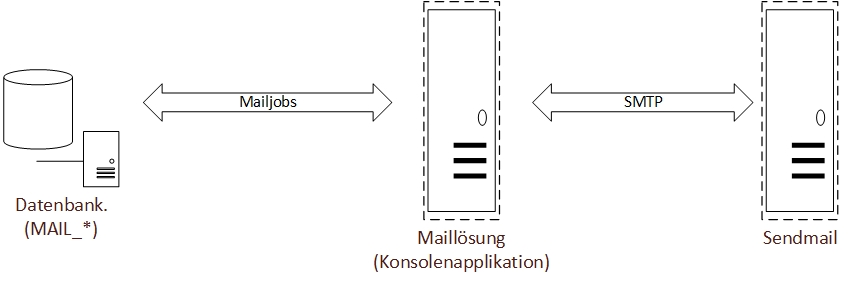
\includegraphics[scale=0.5]{systemaufbau_console_alone.jpg} 
\caption{Teilsystem Konsolen Applikation und Sendmail}
\label{fig:class-hierarchie-email}
\end{figure}


\newpage
\section{Klassenhierarchie}
\label{sec:console-app-class-hierarchie}
Um die Struktur der Konsolen Applikation  zu verstehen wenden wir uns den implementierten Klassenhierarchien der einzelnen Softwarekomponenten wie E-Mail Typen und DAOs (Datenzugriffsobjekte) zu. Diese beiden Softwarekomponenten stellen den Hauptteil der Software dar, daher beginnen wir mit der Analyse dieser Komponenten. 
\subsection{E-Mail Typen}
Einleitend betrachten wir die implementierte Klassenhierarchie der E-Mail Typen mit einem Ausschnitt aus der Klassenhierarchie. Dieser Ausschnitt illustriert sehr gut die vorhandene Struktur der Klassenhierarchie.
\begin{figure}[h]
\centering
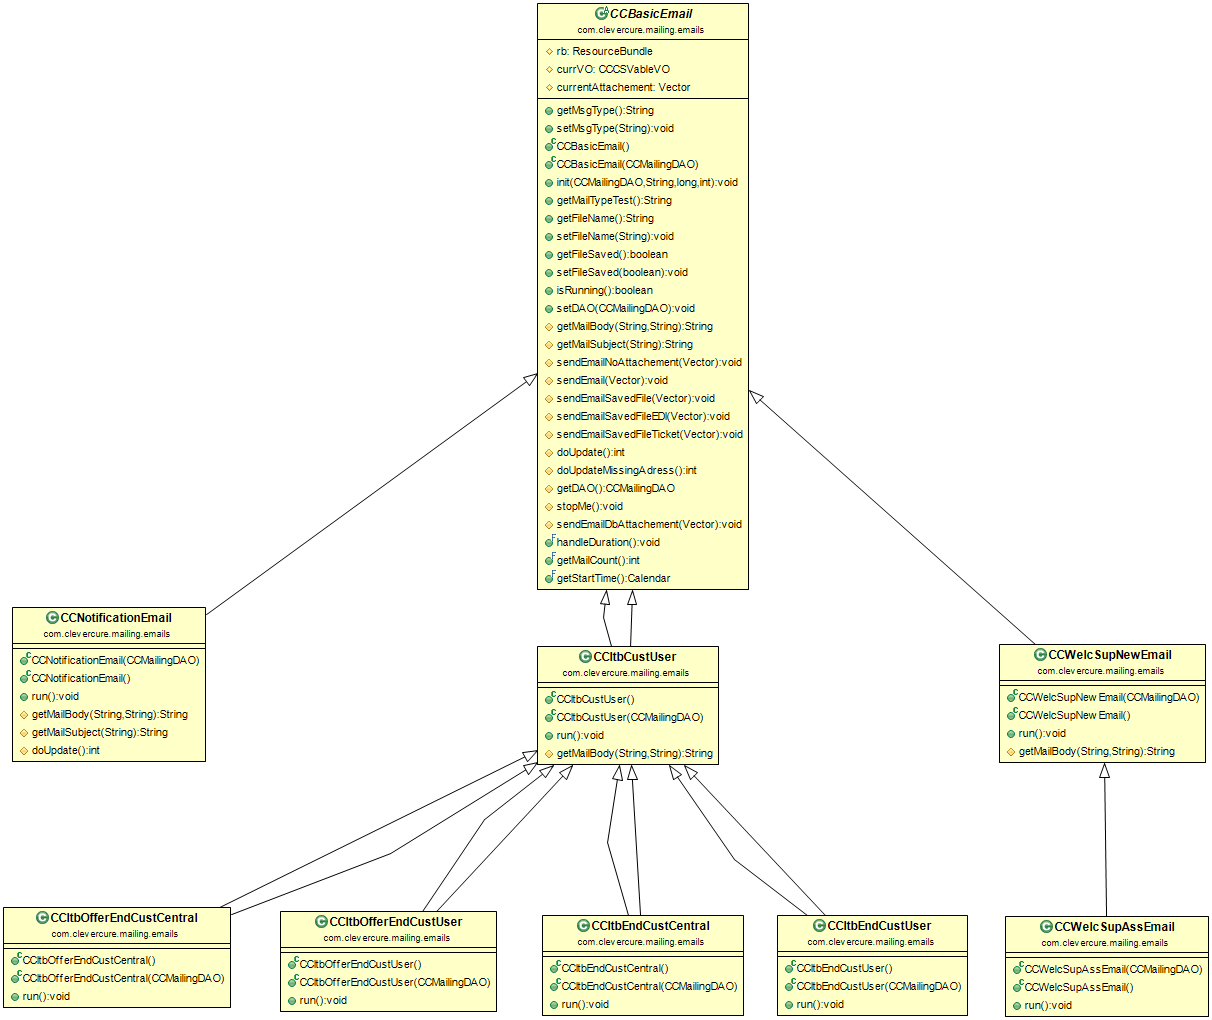
\includegraphics[scale=0.35]{class_diagram_basic_email.png} 
\caption{Die Basisklasse \emph{BasicEmail} mit einigen Implementierungen}
\label{fig:class-hierarchie-email}
\end{figure}

\newpage
Man hat sich hier für das \emph{Factory Method Muster} entschieden wobei die Basisklasse \emph{BasicEmail} eingeführt wurde, welche die gesamte Logik für den Aufbau und Versand einer E-Mail gekapselt und die einzelnen konkreten Implementierungen in Form von abgeleiteten Klassen, die die einzelnen E-Mail Typen darstellen. Wie im Diagramm bei der Klasse \emph{CCItbCustUser} ersichtlich wurden auch E-Mail Typen implementiert, die ihrerseits wieder als Basisklasse dienen für untergeordnete E-Mail Typen. Aufgrund des vergebenen Namens kann man annehmen dass es sich hier um E-Mail Benachrichtigungen für einen Benutzer eines Kunden des Moduls ITB handelt, die man versucht hat zu gruppieren.\\
Die Gruppierung wurde hier durch Einführung einer eigenen Vererbungshierarchie auf Basis einer eingeführten Basisklasse \emph{CCItbCustUser}, die ihrerseits die eigentliche Basisklasse \emph{BasicEmail} weg abstrahiert, realisiert.\\

An sich ist dies kein schlechter Ansatz jedoch erwarte ich mir von einer konkreten Implementierung, dass diese auch ein gewisses Maß an Logik beinhaltet, die das Factory-Method Muster rechtfertigt, jedoch ist dies in den meisten Fällen nicht der Fall, wie im nächsten Punkt beschrieben wird. Solche Klassenhierarchien einzuführen nur um verschiedene Datentypen zu erhalten, welche einen E-Mail Typ definieren, welcher nicht einmal in den angeschlossenen Systemen verwendet wird sondern nur innerhalb dieser Konsolen Applikation finde ich übertrieben. Es gibt weitaus einfachere, weniger aufwendige und Code produzierende Ansätze mit denen E-Mail Typen abgebildet werden können.

\newpage
\subsection{Datenzugriffsobjekt(e)}
Nachdem wir die Klassenhierarchie der E-Mail Typen analysiert haben wenden wir uns nun der Datenbankzugriffsschicht zu, die mit einem einzigen DAO (Datenzugriffsobjekt) implementiert wurde.
\begin{figure}[h]
\centering
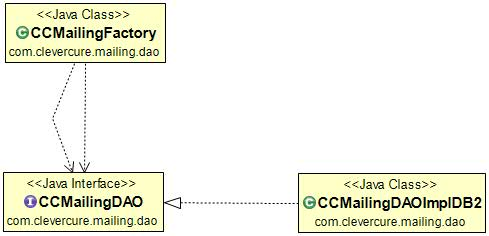
\includegraphics[scale=0.5]{cc_mail_dao.jpg} 
\caption{Die \emph{CCMailingDAOImplDB2} Implementierung mit seinem Interface \emph{CCMailingDAO} mit seiner Factory \emph{CCMailingFactory}}
\label{fig:class-hierarchie-email}
\end{figure}
\ \\
Obwohl man eine Klassenhierarchie für die E-Mail Typen eingeführt hat, hat man dies bei den DAOs (Datenzugriffsobjekte) nicht getan. Es gibt also eine einzige DAO Implementierung, die alle Datenbankabfragen über alle E-Mail Typen hinweg beinhaltet und diese über eindeutige Methodennamen identifiziert. Des Weiteren wurde zwar eine Factory für dieses DAO eingeführt, aber eine Factory für ein DAO mit \emph{Class.forName("*.DaoImplDb2")} erscheint fast sinnlos, obwohl man hier noch die Begründung finden könnte, dass diese Factory eingeführt wurde um zumindest die konkrete Datenbank zu abstrahieren und die Möglichkeit zu schaffen die DAO Implementierung für DB2 auf z.B.: Oracle zu ändern. Man würde hier erwarten das die DAO Implementierung kontextabhängig - also auf Modulebene - implementiert worden wären und dass die Factory dynamisch mit der zu verwendenden Implementierung initialisiert werden kann, also parametriebar ist. Dann wäre es aber auch erforderlich die Datenbank spezifischen Implementierungen über ein eigenes Artifakt zur Verfügung zu stellen und nicht das alle Ressourcen sich innerhalb ein und desselben Artifakts befinden.

\newpage
\section{Implementierung}
Da wir nun die Klassenhierarchien kennen gelernt haben wenden wir uns deren Implementierung zu. Im folgenden werden die Implementierungen der Klasse \emph{CCItbCustUser} und dessen Ableitungen diskutiert. Im Punkt~\ref{sec:console-app-class-hierarchie} wurde behauptet dass diese Ableitungen eingeführt wurden um E-Mail Typen zu gruppieren. Man könnte aber auch davon ausgehen dass diese eigene Vererbungshierarchie eingeführt wurde um Funktionalitäten für die einzelnen E-Mails zu kapseln. Analysieren wir nun diese Implementierungen um zu sehen welche Funktionalitäten in einen E-Mail Typ implementiert wurden. \\



// TODO: Add source of 'CCItbCustUser' and its decendants. \\
// TODO: CCItbCustUser \\\\


\newpage

Im folgenden wird das existierende Design der Implementierung in den drei Bereichen
\begin{enumerate}
	\item \emph{Client-API}\\
	      Wie versenden bzw. generieren die Systeme die E-Mails
	\item \emph{Datenbank Integration}\\
	      Wie ist das Datenbankdesign und welche Daten werden gespeichert und warum
	\item \emph{E-Mail Vorlagen}\\
	      Wie werden die Inhalte der E-Mail generiert bzw. erstellt.
\end{enumerate}
Da der Mailversand in Java verhältnismäßig einfach ist wird auf diesen Teil nicht genauer eingegangen sehr wohl aber die Funktionalität im weiteren Verlauf dieser Arbeit diskutiert. \
Die oben genannten drei Unterteilungen stellen die Hauptteile der Maillösung dar und werden auch in einem neuen Design so benötigt ohne Rücksichtnahme auf die konkrete Art der Implementierung.
\begin{figure}[h]
\centering
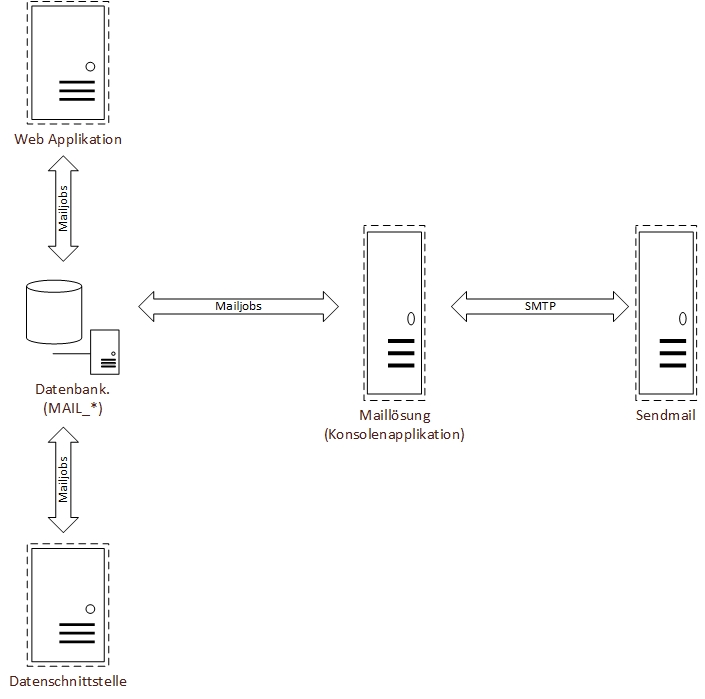
\includegraphics[scale=0.40]{Systemaufbau_alt.jpg} %{CS0031}
\caption{Diese Abbildung zeigt den konzeptionellen Aufbau der existierenden Maillösung und den jetzigen Kommunikationsweg zwischen den Systemteilnehmern}
\label{fig:systemaufbau-alt}
\end{figure}
\newpage
In dieser Abbildung können wir sehen dass es nur einen Kommunikationsweg zwischen den Systemteilnehmer gibt und zwar die Kommunikation über die Datenbank. Dies bedeutet es werden sogenannte Mailjobs erstellt, die einen Eintrag in einer Tabelle der Datenbank darstellen, welche alle Daten für die E-Mail zur Verfügung stellen und von der Maillösung ausgelesen und verarbeitet werden.\\
Hierbei enthält die Maillösung alle Vorlagen für alle implementierten E-Mails und SQL Abfragen, die die Daten aus der Datenbank auslesen und diese ausgelesenen Daten als Parameter and das Vorlagensystem weitergibt damit dieses die tatsächliche E-Mail Nachricht erstellen kann. Hierbei ist die Aktualität der Daten kritisch, da die E-Mail zeitversetzt zum erstellten Mailjob generiert wird und sich dadurch auch die Daten, die aus der Datenbank ausgelesen werden, sich zwischenzeitlich ändern könnten. Ebenso müssen die Daten separat und meistens erneut aus der Datenbank ausgelesen werden, obwohl in den meisten Fällen die Daten beim Erstellen des Mailjobs bereits vorhanden und vor allem zu diesem Zeitpunkt auch aktuell waren. Es gibt zwar Fälle in denen zeitgesteuert E-Mails generiert werden, wie z.B.: einmal täglich Lieferverzugsmeldungen, in denen der aktuelle Status der Datenbank eine Rolle spielt. Dieser Typ der E-Mails stellt jedoch im Verhältnis zu den \emph{'sofort versendeten'} E-Mails nur einen kleinen Prozentanteil dar und hier ist das Problem der Aktualität der verwendeten Daten nicht vorhanden. Bezüglich der Aktualität der Daten sei noch angemerkt dass das erneute Versenden einer E-Mail im bestehenden System nicht mit konsistent Daten möglich ist, da die Daten jedes mal erneut aus der Datenbank ausgelesen werden und der ursprüngliche Zustand der Daten nicht garantiert zur Verfügung steht, da diese sich zwischenzeitlich hätten ändern können, was auch nicht nachvollziehbar wäre.
\subsection{Client-API}
Da die Kommunikation ausschließlich über die Datenbank erfolgt ist eine echte Client API nicht vorhanden. Alle Systeme implementieren das Erstellen der Mailjob Einträge selbstständig und es wird keine gemeinsame Client API verwendet, was einen gewissen Grad der Inkonsistenz bei Änderungen der Datenstruktur sowie der Semantik der Daten mit sich bringt. Als Beispiel wird hier die Semantik der einzelnen Spalten angeführt, die zwar technisch sich innerhalb einer Datentyp Domain befinden, sich die semantische Bedeutung der enthaltenen Daten aber unterscheidet. Dies ist zwar Teil der Datenbank Integration aber die Tatsache dass diese Semantik rein innerhalb der Applikation abgebildet werden kann und nicht über die Datenbankfunktionalitäten wie z.B.: Fremdschlüssel wird dieser Teil hier diskutiert. Da die Maillösung über SQL Abfragen die Daten für die E-Mail Nachricht erhält müssen auch Parameter bereitgestellt werden, die in der SQL Abfrage gesetzt werden. Diese Parameter wurden \emph{'generisch'} über eine festgesetzte Anzahl von Tabellenspalten abgebildet, dessen enthaltene Daten je nach E-Mailtyp anders interpretiert werden. Es kann also sein das ein Eintrag einer Tabellen für die Spalte \emph{COL\_1} einen String enthält mit dem Wert \emph{'Thomas Herzog'} und ein anderer Eintrag einen string mit dem Wert \emph{'14'} der in der SQL Abfrage aber als Integer Datentyp behandelt wird. Die Systeme die Mailjobs erzeugen müssen sich also dem Kontext einer E-Mail bewusst sein, sowie müssen berücksichtigen, dass die richten Spalten der Tabelle \emph{MAIL\_JOB} mit den richtigen Daten befüllt werden, wobei auch beachtet werden muss in welchen Datentyp der Datensatz in weiterer Folge durch die Mailösung interpretiert wird.\\
Dies ist in meinen Augen sehr inkonsistent und fehleranfällig und hat auch schon einige Probleme verursacht.\\\\
\begin{figure}[h]
\centering
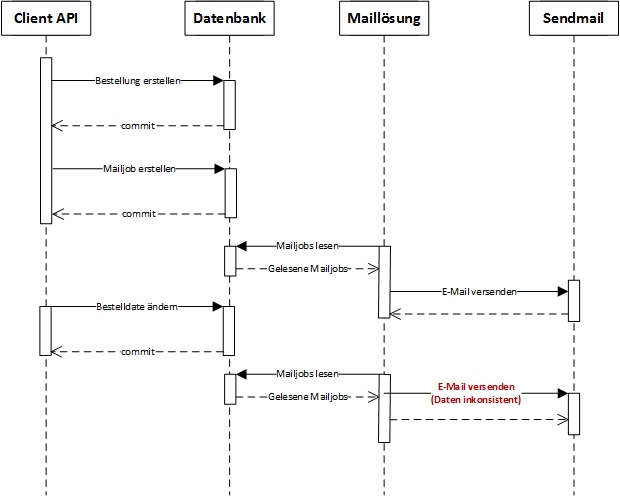
\includegraphics[scale=0.70]{Emailvesand_Client_Api.jpg}
\caption{Diese Abbildung zeigt das Problem der inkonsistenten Daten beim erneuten E-Mailversand einer bereits versendeten E-Mail, mit dem Beispiel einer angelegten und anschließend geänderten Bestellung, auf}
\label{fig:systemaufbau-alt}
\end{figure}
\newpage



\subsection{Datenbank Integration}
\subsection{E-Mail Vorlagen}
\section{Soll-System}
\subsection{Client-API}
\subsection{Datenbank Integration}
\subsection{E-Mail Vorlagen}

\section{Arbeiten in Englisch}
\label{sec:englisch}
